\documentclass[twoside]{book}

% Packages required by doxygen
\usepackage{fixltx2e}
\usepackage{calc}
\usepackage{doxygen}
\usepackage[export]{adjustbox} % also loads graphicx
\usepackage{graphicx}
\usepackage[utf8]{inputenc}
\usepackage{makeidx}
\usepackage{multicol}
\usepackage{multirow}
\PassOptionsToPackage{warn}{textcomp}
\usepackage{textcomp}
\usepackage[nointegrals]{wasysym}
\usepackage[table]{xcolor}

% Font selection
\usepackage[T1]{fontenc}
\usepackage[scaled=.90]{helvet}
\usepackage{courier}
\usepackage{amssymb}
\usepackage{sectsty}
\renewcommand{\familydefault}{\sfdefault}
\allsectionsfont{%
  \fontseries{bc}\selectfont%
  \color{darkgray}%
}
\renewcommand{\DoxyLabelFont}{%
  \fontseries{bc}\selectfont%
  \color{darkgray}%
}
\newcommand{\+}{\discretionary{\mbox{\scriptsize$\hookleftarrow$}}{}{}}

% Page & text layout
\usepackage{geometry}
\geometry{%
  a4paper,%
  top=2.5cm,%
  bottom=2.5cm,%
  left=2.5cm,%
  right=2.5cm%
}
\tolerance=750
\hfuzz=15pt
\hbadness=750
\setlength{\emergencystretch}{15pt}
\setlength{\parindent}{0cm}
\setlength{\parskip}{3ex plus 2ex minus 2ex}
\makeatletter
\renewcommand{\paragraph}{%
  \@startsection{paragraph}{4}{0ex}{-1.0ex}{1.0ex}{%
    \normalfont\normalsize\bfseries\SS@parafont%
  }%
}
\renewcommand{\subparagraph}{%
  \@startsection{subparagraph}{5}{0ex}{-1.0ex}{1.0ex}{%
    \normalfont\normalsize\bfseries\SS@subparafont%
  }%
}
\makeatother

% Headers & footers
\usepackage{fancyhdr}
\pagestyle{fancyplain}
\fancyhead[LE]{\fancyplain{}{\bfseries\thepage}}
\fancyhead[CE]{\fancyplain{}{}}
\fancyhead[RE]{\fancyplain{}{\bfseries\leftmark}}
\fancyhead[LO]{\fancyplain{}{\bfseries\rightmark}}
\fancyhead[CO]{\fancyplain{}{}}
\fancyhead[RO]{\fancyplain{}{\bfseries\thepage}}
\fancyfoot[LE]{\fancyplain{}{}}
\fancyfoot[CE]{\fancyplain{}{}}
\fancyfoot[RE]{\fancyplain{}{\bfseries\scriptsize Generated by Doxygen }}
\fancyfoot[LO]{\fancyplain{}{\bfseries\scriptsize Generated by Doxygen }}
\fancyfoot[CO]{\fancyplain{}{}}
\fancyfoot[RO]{\fancyplain{}{}}
\renewcommand{\footrulewidth}{0.4pt}
\renewcommand{\chaptermark}[1]{%
  \markboth{#1}{}%
}
\renewcommand{\sectionmark}[1]{%
  \markright{\thesection\ #1}%
}

% Indices & bibliography
\usepackage{natbib}
\usepackage[titles]{tocloft}
\setcounter{tocdepth}{3}
\setcounter{secnumdepth}{5}
\makeindex

% Hyperlinks (required, but should be loaded last)
\usepackage{ifpdf}
\ifpdf
  \usepackage[pdftex,pagebackref=true]{hyperref}
\else
  \usepackage[ps2pdf,pagebackref=true]{hyperref}
\fi
\hypersetup{%
  colorlinks=true,%
  linkcolor=blue,%
  citecolor=blue,%
  unicode%
}

% Custom commands
\newcommand{\clearemptydoublepage}{%
  \newpage{\pagestyle{empty}\cleardoublepage}%
}

\usepackage{caption}
\captionsetup{labelsep=space,justification=centering,font={bf},singlelinecheck=off,skip=4pt,position=top}

%===== C O N T E N T S =====

\begin{document}

% Titlepage & ToC
\hypersetup{pageanchor=false,
             bookmarksnumbered=true,
             pdfencoding=unicode
            }
\pagenumbering{alph}
\begin{titlepage}
\vspace*{7cm}
\begin{center}%
{\Large My Project }\\
\vspace*{1cm}
{\large Generated by Doxygen 1.8.13}\\
\end{center}
\end{titlepage}
\clearemptydoublepage
\pagenumbering{roman}
\tableofcontents
\clearemptydoublepage
\pagenumbering{arabic}
\hypersetup{pageanchor=true}

%--- Begin generated contents ---
\chapter{C\+S202\+\_\+\+F21\+\_\+\+Group\+\_\+\+Project}
\label{index}\hypertarget{index}{}\section*{Group 3}

Project Level\+: Basic

{\bfseries Tasks\+:}

Project Members\+: Tania Jaswal, Austin Ah Mau and Donavin Phelps

U\+I/\+D\+O\+X\+Y\+G\+EN\+: Tania Jaswal

File Loading(\+W\+A\+V)\+: Donavin Phelps

Effects/\+Filters(Processor)\+: Austin Ah Mau

{\bfseries U\+ML Diagram\+:}

{\bfseries Issue incountered during this project\+:}

{\bfseries Challenges incountered during this project\+:}

{\bfseries Building Application\+:} 
\chapter{Hierarchical Index}
\section{Class Hierarchy}
This inheritance list is sorted roughly, but not completely, alphabetically\+:\begin{DoxyCompactList}
\item \contentsline{section}{Processable}{\pageref{classProcessable}}{}
\begin{DoxyCompactList}
\item \contentsline{section}{Normalization}{\pageref{classNormalization}}{}
\begin{DoxyCompactList}
\item \contentsline{section}{Gain}{\pageref{classGain}}{}
\end{DoxyCompactList}
\end{DoxyCompactList}
\item \contentsline{section}{UI}{\pageref{classUI}}{}
\item \contentsline{section}{Wav}{\pageref{classWav}}{}
\item \contentsline{section}{wav\+\_\+header}{\pageref{structwav__header}}{}
\end{DoxyCompactList}

\chapter{Class Index}
\section{Class List}
Here are the classes, structs, unions and interfaces with brief descriptions\+:\begin{DoxyCompactList}
\item\contentsline{section}{\hyperlink{classWav}{Wav} }{\pageref{classWav}}{}
\item\contentsline{section}{\hyperlink{structwav__header}{wav\+\_\+header} }{\pageref{structwav__header}}{}
\end{DoxyCompactList}

\chapter{Class Documentation}
\hypertarget{classGain}{}\section{Gain Class Reference}
\label{classGain}\index{Gain@{Gain}}


Inheritance diagram for Gain\+:

\hypertarget{classNormalization}{}\section{Normalization Class Reference}
\label{classNormalization}\index{Normalization@{Normalization}}


Inheritance diagram for Normalization\+:
% FIG 0


Collaboration diagram for Normalization\+:
% FIG 1
\subsection*{Public Member Functions}
\begin{DoxyCompactItemize}
\item 
\mbox{\Hypertarget{classNormalization_a59c6ac0b235429f48212236fdc6f6f44}\label{classNormalization_a59c6ac0b235429f48212236fdc6f6f44}} 
void {\bfseries get\+Data} (\hyperlink{classWav}{Wav} sound)
\item 
\mbox{\Hypertarget{classNormalization_a7666aa086ded5e86b4b5c330e49bab26}\label{classNormalization_a7666aa086ded5e86b4b5c330e49bab26}} 
void {\bfseries process} ()
\item 
\mbox{\Hypertarget{classNormalization_a17e9a95b24923be2524fd790dae5b752}\label{classNormalization_a17e9a95b24923be2524fd790dae5b752}} 
std\+::vector$<$ float $>$ {\bfseries get\+Normal} ()
\end{DoxyCompactItemize}


The documentation for this class was generated from the following files\+:\begin{DoxyCompactItemize}
\item 
normalization.\+h\item 
normalization.\+cpp\end{DoxyCompactItemize}

\hypertarget{classProcessable}{}\section{Processable Class Reference}
\label{classProcessable}\index{Processable@{Processable}}


Inheritance diagram for Processable\+:
\nopagebreak
\begin{figure}[H]
\begin{center}
\leavevmode
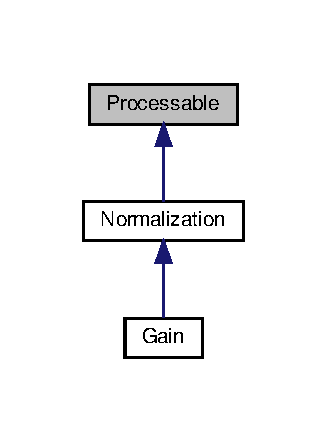
\includegraphics[width=157pt]{da/d78/classProcessable__inherit__graph}
\end{center}
\end{figure}
\subsection*{Public Member Functions}
\begin{DoxyCompactItemize}
\item 
\mbox{\Hypertarget{classProcessable_a56c36f88f509d6030d06d58f6bf9d8df}\label{classProcessable_a56c36f88f509d6030d06d58f6bf9d8df}} 
virtual void {\bfseries process} ()=0
\end{DoxyCompactItemize}


The documentation for this class was generated from the following files\+:\begin{DoxyCompactItemize}
\item 
processable.\+h\item 
processable.\+cpp\end{DoxyCompactItemize}

\hypertarget{classUI}{}\section{UI Class Reference}
\label{classUI}\index{UI@{UI}}
\subsection*{Public Member Functions}
\begin{DoxyCompactItemize}
\item 
\mbox{\Hypertarget{classUI_ade684e1af6cdcc9ad9a9f4049294d5f7}\label{classUI_ade684e1af6cdcc9ad9a9f4049294d5f7}} 
void {\bfseries Start\+Option} ()
\item 
\mbox{\Hypertarget{classUI_aac4ec5438f211612234d8f9be155eaf2}\label{classUI_aac4ec5438f211612234d8f9be155eaf2}} 
std\+::string {\bfseries Input\+Filename} ()
\item 
\mbox{\Hypertarget{classUI_a81e54c22892df22c6b67a10e4d0e58e6}\label{classUI_a81e54c22892df22c6b67a10e4d0e58e6}} 
bool {\bfseries check\+Input} (std\+::string input)
\item 
\mbox{\Hypertarget{classUI_a8f4736f8a5097a1f234678ac85544b28}\label{classUI_a8f4736f8a5097a1f234678ac85544b28}} 
void {\bfseries Invalid\+File\+Name} ()
\item 
\mbox{\Hypertarget{classUI_a8d1d1f3df8d204f641c085a4d3730c1b}\label{classUI_a8d1d1f3df8d204f641c085a4d3730c1b}} 
void {\bfseries Exit\+Option} ()
\item 
\mbox{\Hypertarget{classUI_ad5a96cf0e114c4dac4a4d7958dd98c4a}\label{classUI_ad5a96cf0e114c4dac4a4d7958dd98c4a}} 
std\+::string {\bfseries Output\+File\+Name} ()
\end{DoxyCompactItemize}
\subsection*{Static Public Member Functions}
\begin{DoxyCompactItemize}
\item 
\mbox{\Hypertarget{classUI_a3af627515035a845a98b24d7463da5dc}\label{classUI_a3af627515035a845a98b24d7463da5dc}} 
static std\+::string {\bfseries Processor\+Options} ()
\end{DoxyCompactItemize}


The documentation for this class was generated from the following files\+:\begin{DoxyCompactItemize}
\item 
U\+I.\+h\item 
U\+I.\+cpp\end{DoxyCompactItemize}

\hypertarget{classWav}{}\section{Wav Class Reference}
\label{classWav}\index{Wav@{Wav}}
\subsection*{Public Member Functions}
\begin{DoxyCompactItemize}
\item 
\mbox{\Hypertarget{classWav_a1c4230cec49d30147a5b8a1950083f7c}\label{classWav_a1c4230cec49d30147a5b8a1950083f7c}} 
void {\bfseries read\+File} (const std\+::string \&file\+Name)
\end{DoxyCompactItemize}


The documentation for this class was generated from the following files\+:\begin{DoxyCompactItemize}
\item 
Wav.\+h\item 
wav.\+cpp\end{DoxyCompactItemize}

\hypertarget{structwav__header}{}\section{wav\+\_\+header Struct Reference}
\label{structwav__header}\index{wav\+\_\+header@{wav\+\_\+header}}
\subsection*{Public Attributes}
\begin{DoxyCompactItemize}
\item 
\mbox{\Hypertarget{structwav__header_a977b8193bf1f39dbd815c6210f0bb6c6}\label{structwav__header_a977b8193bf1f39dbd815c6210f0bb6c6}} 
char {\bfseries riff\+\_\+header} \mbox{[}4\mbox{]}
\item 
\mbox{\Hypertarget{structwav__header_a89a86a26a94e726411e34517bfc9105e}\label{structwav__header_a89a86a26a94e726411e34517bfc9105e}} 
int {\bfseries wav\+\_\+size}
\item 
\mbox{\Hypertarget{structwav__header_a0dc0cff34ad7fe5e59c5cbcee1640354}\label{structwav__header_a0dc0cff34ad7fe5e59c5cbcee1640354}} 
char {\bfseries wave\+\_\+header} \mbox{[}4\mbox{]}
\item 
\mbox{\Hypertarget{structwav__header_a4039d1e8e91d7940aa45a29aad27b4ce}\label{structwav__header_a4039d1e8e91d7940aa45a29aad27b4ce}} 
char {\bfseries fmt\+\_\+header} \mbox{[}4\mbox{]}
\item 
\mbox{\Hypertarget{structwav__header_a5fb4363d52bbff51ca2e8884408208c6}\label{structwav__header_a5fb4363d52bbff51ca2e8884408208c6}} 
int {\bfseries fmt\+\_\+chunk\+\_\+size}
\item 
\mbox{\Hypertarget{structwav__header_a94c9ee0387f846c47eb9e97636994d93}\label{structwav__header_a94c9ee0387f846c47eb9e97636994d93}} 
short {\bfseries audio\+\_\+format}
\item 
\mbox{\Hypertarget{structwav__header_a625d84de0f598e50c072d725f6e3b6b8}\label{structwav__header_a625d84de0f598e50c072d725f6e3b6b8}} 
short {\bfseries num\+\_\+channels}
\item 
\mbox{\Hypertarget{structwav__header_a0632019c676aa88f0351c0ab11461de0}\label{structwav__header_a0632019c676aa88f0351c0ab11461de0}} 
int {\bfseries sample\+\_\+rate}
\item 
\mbox{\Hypertarget{structwav__header_a8330740d45200d6aee4ba54fc0d834d8}\label{structwav__header_a8330740d45200d6aee4ba54fc0d834d8}} 
int {\bfseries byte\+\_\+rate}
\item 
\mbox{\Hypertarget{structwav__header_a2672b73c81973008677db6349fbc232a}\label{structwav__header_a2672b73c81973008677db6349fbc232a}} 
short {\bfseries sample\+\_\+alignment}
\item 
\mbox{\Hypertarget{structwav__header_a63fa60069060bae97c8a64c5b37afa23}\label{structwav__header_a63fa60069060bae97c8a64c5b37afa23}} 
short {\bfseries bit\+\_\+depth}
\item 
\mbox{\Hypertarget{structwav__header_ae43fac12459053e98a80e3879c5cd2a7}\label{structwav__header_ae43fac12459053e98a80e3879c5cd2a7}} 
char {\bfseries data\+\_\+header} \mbox{[}4\mbox{]}
\item 
\mbox{\Hypertarget{structwav__header_a3eeeca270947eab7c7aaee61bbee9b0e}\label{structwav__header_a3eeeca270947eab7c7aaee61bbee9b0e}} 
int {\bfseries data\+\_\+bytes}
\end{DoxyCompactItemize}


The documentation for this struct was generated from the following file\+:\begin{DoxyCompactItemize}
\item 
wav\+Header.\+h\end{DoxyCompactItemize}

%--- End generated contents ---

% Index
\backmatter
\newpage
\phantomsection
\clearemptydoublepage
\addcontentsline{toc}{chapter}{Index}
\printindex

\end{document}
